\documentclass[10pt]{beamer}

%%
%% Examples in comment for including certain frames
%%
%%\includeonlyframes{outline,overview}
%%
%% This will include only the frames with labels outline and overview
%%
%% \begin{frame}[label=overview]
%%
%% \end{frame}

%%\includeonlyframes{hulpmiddelen}

\usepackage{ucs}
\usepackage[utf8x]{inputenc}
\usepackage{beamerthemebars}

\usepackage{subfigure}
\usepackage[english]{babel}
\usepackage{graphicx}
\usepackage{amssymb}% For \checkmark
\usepackage{pifont}% for \ding{'-code or "-code}
\usepackage{pgfgantt}

\title[Plan]{An overview of the project plan\\ for rebuilding WickedXMAS}
\subtitle[Overview]{An Overview}
\author[Team33]{Team33: Guus Bonnema, Jeroen Kleijn, Stefan Versluys}
\date{18-10-2014}
\institute[OU nl]{Open University The Netherlands}
%%\logo{\includegraphics[scale=.25]{oulogo.pdf}}    <- OU has no logo that I could download


\begin{document}

%%%%%%%%%%%%%%%%%%%%%%%%%%%%%%%%%%%%
\newcommand{\xmas}{x\textsc{mas}}%
\newcommand{\ok}{$\checkmark$}

%%%%%%%%%%%%%%%%%%%%%%%%%%%%%%%%%%%%
\mode<presentation>

\frame{\maketitle}   % <-- generate frame with title.

%%%%%%%%%%%%%%%%%%%%%%%%%%%%%%%%%%%%
%%
%% This is part of quick-plan.tex
%%
\begin{frame}
    \section{Project}

    Guus Bonnema
\end{frame}

\begin{frame}[label=outline]
    \frametitle{Outline}
    \tableofcontents[pausesections]
\end{frame}



\begin{frame}[label=opdracht]{Overview deel 1}{Project Opdracht}

    \begin{columns}
        \begin{column}<1->{.4\textwidth}
	    Project opdracht

	    \begin{itemize}
		\item business case
		\item vision
		\item Challanges and goals (*)
		\item Succesfactoren (*)
		\item Risico (*)
	    \end{itemize}
        \end{column}
        \begin{column}<2->{.4\textwidth}
	    Project uitvoering

	    \begin{itemize}
		\item iteratief
		\item tijdgedreven
		\item samenwerking $\rightarrow$ rolverdeling
		\item hulpmiddelen (*)
	    \end{itemize}
        \end{column}


    \end{columns}



\end{frame}

\begin{frame}[label=challanges]{Overview deel 2}{Project Uitvoering}

    \begin{columns}[t]
        \begin{column}<1->{.5\textwidth}
	    Uitdagingen
	    \begin{description}
	        \item[Platformen] {\tiny MS Windows, Mac en Linux.}
	        \item[Integratie] {\tiny Verficatie tools.}
	        \item[Onderhoud] {\tiny Velen gaan dit onderhoud plegen.}
		\item[Uitbreiding] {\tiny researchtool $\rightarrow$ uitbreidbaar.}
		\item[Functie] {\tiny als WickedXMAS}
	    \end{description}


        \end{column}
        \begin{column}<2->{.4\textwidth}
	    Succes factoren
	    \begin{itemize}
	        \item {\tiny design tool te gebruiken op alle platformen}
	        \item {\tiny functioneert gelijkwaardig aan WickedXMas}
	    \end{itemize}
	    Groot success
	    \begin{itemize}
	        \item {\tiny validatie en verificatie optioneel, wijzigbaar}
	        \item {\tiny primitieven defini\"{e}ren}
	    \end{itemize}
        \end{column}

    \end{columns}


\end{frame}

\begin{frame}[fragile]{Overview deel 1}{Risico's}

    Bijna alle risico's hebben een maatregel


    {\tiny
    \begin{tabular}{|c|c|p{15em}|p{25em}|c|c|}
     \hline
{\bf } & {\bf nr} & {\bf Risico} & {\bf Toelichting} & {\bf Kans} & {\bf Ernst} \\\hline
  \ok & 1 & Stakeholders zijn niet op het gewenste moment beschikbaar  & De opdrachtgever en de begeleider hebben een beperkte tijd
					beschikbaar. De andere stakeholders zijn niet beschikbaar. & hoog & middel \pause\\\hline
  \ok & 2 & Project verloopt niet goed door gebrek aan Agile ervaring & De teamleden hebben vooral ervaring
	    met waterval projecten. & hoog & middel \\\hline\pause
  \ok & 3 & Vertraging van activiteiten door trage support (OU) & De support van de
	    OU lijkt niet al te voortvarend. Dit kan problemen veroorzaken. & middel & laag \pause\\\hline
  \ok & 4 & Er is meer tijd nodig dan gedacht om de materiekennis op te doen & Het kost tijd om de bestaande verificatietools en de achterliggende
					xmas-materie op te nemen. & laag & middel \pause\\\hline
  \ok & 5 & Communicatieproblemen treden op door geografische spreiding & Het team woont te ver uit elkaar om face to face meetings te
				organiseren voor overleg tijdens het project. & middel & middel \pause\\\hline
  \ok & 6 & Ontstaan van structuurverval bij ontwikkeling & Bij het toevoegen van functionaliteit is structuurverval een
				natuurlijk gevolg. & middel & hoog \pause\\\hline
  \ok & 7 & Weinig ervaring met c++ leidt tot lagere kwaliteit en bruikbaarheid van de opgeleverde software & Het team heeft maar \'e\'en ervaren C++ programmeur en deze
  heeft vooral ervaring met embedded systems. Dit gebrek aan ervaring kan er toe leiden dat de softwareontwikkeling vertraging oploopt. In de
  beschikbare tijd kunnen minder features worden ontwikkeld dan oorspronkelijk gepland. Verkeerd gebruik (bad practices) van de programmeertaal kan een bedreiging zijn
  voor de softwarekwaliteit. & middel & hoog \pause\\\hline
  \ding{"38} & 8 & Fouten in ontwerp & Bij het ontwerpen kunnen fouten ontstaan die de controles niet ontdekken. & laag & hoog \\\hline

    \end{tabular}

    }

\end{frame}

\begin{frame}[fragile,label=hulpmiddelen]{Overview deel 2}{Hulpmiddelen}

    Hulpmiddelen

    \begin{columns}[c]
	\begin{column}{10em}
	    \begin{itemize}
		\item<1> git
		\item<1> github
		\item<2> google group
		\item<3> agilefant
	    \end{itemize}
	\end{column}

	\begin{column}{30em}
	    \begin{center}
		\begin{tabular}{l}
		    \includegraphics<1>[height=.25\textheight]{github-example}\\
		    \includegraphics<2>[height=.25\textheight]{google-groups-example}\\
		    \includegraphics<3>[height=.25\textheight]{agilefant-example}\\
		\end{tabular}
	    \end{center}
	\end{column}


    \end{columns}


\end{frame}
%%
%% This is part of quick-plan.tex
%%
\begin{frame}
    \section{Process}
    Stefan Versluys
\end{frame}

\begin{frame}[label=process1]{DAD Process}{Betekenis}
	Disciplined Agile Delivery?
	\begin{itemize}[<+->]
	 	\item Leergericht
		\item Agile
		\item Hybride
		\item Oplossing boven software
		\item Doel gedreven
		\item Risico en waarde prioriteit
	\end{itemize}
\end{frame}

\begin{frame}[fragile]{DAD Process}{Indeling fasen}
	\begin{enumerate}
	\item<1-> Inceptiefase
		\begin{itemize}
		\item 2 iteraties
			$\rightarrow$ Planning, domeinanalyse, visie.
		\end{itemize}
	\item<2-> Constructiefase
		\begin{itemize}
		\item 6 iteraties
			$\rightarrow$ Architectuur, prototype, documentatie.
		\end{itemize}
	\item<3-> Transitiefase
		\begin{itemize}
		\item 1 iteratie
			$\rightarrow$ Presentatie, oplossing.
		\end{itemize}		
	\end{enumerate}  
\end{frame}


\begin{frame}[label=process2]{DAD Process}{Life cylce}
    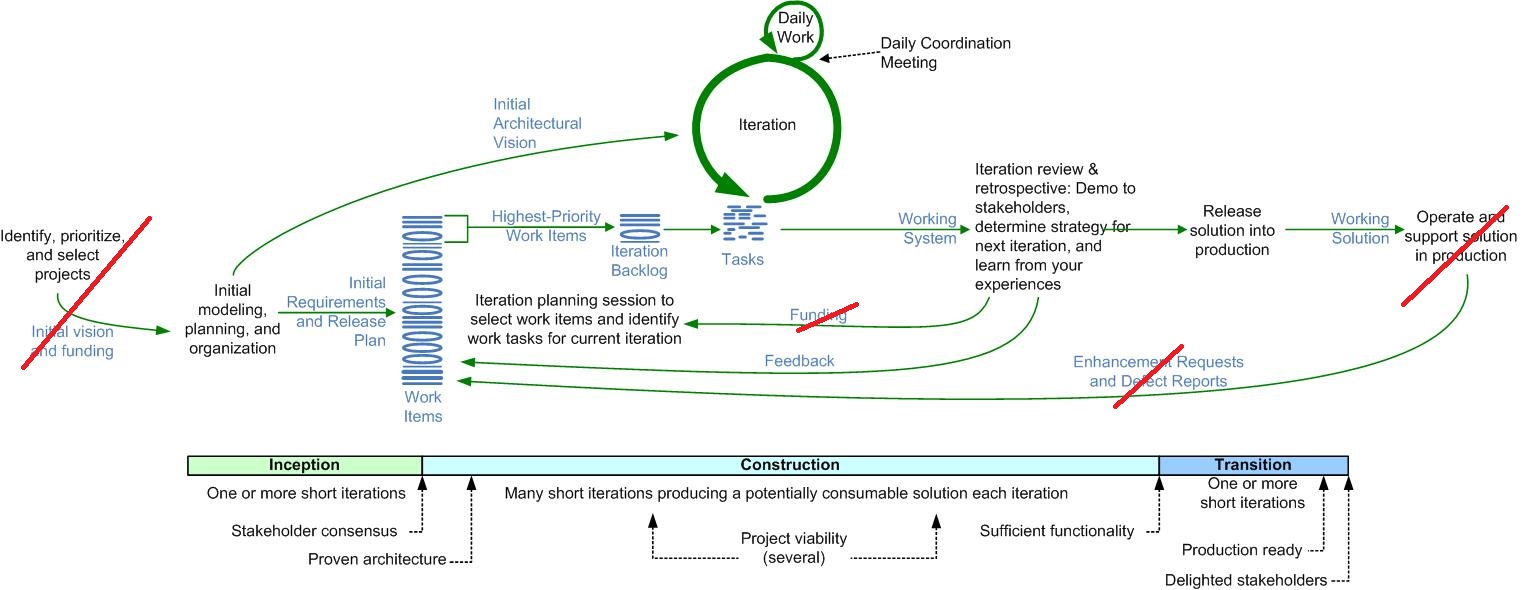
\includegraphics[width = .9\textwidth]{dadLifecycleUP2}
\end{frame}

\begin{frame}[label=process2]{DAD Process}{Life cylce}
    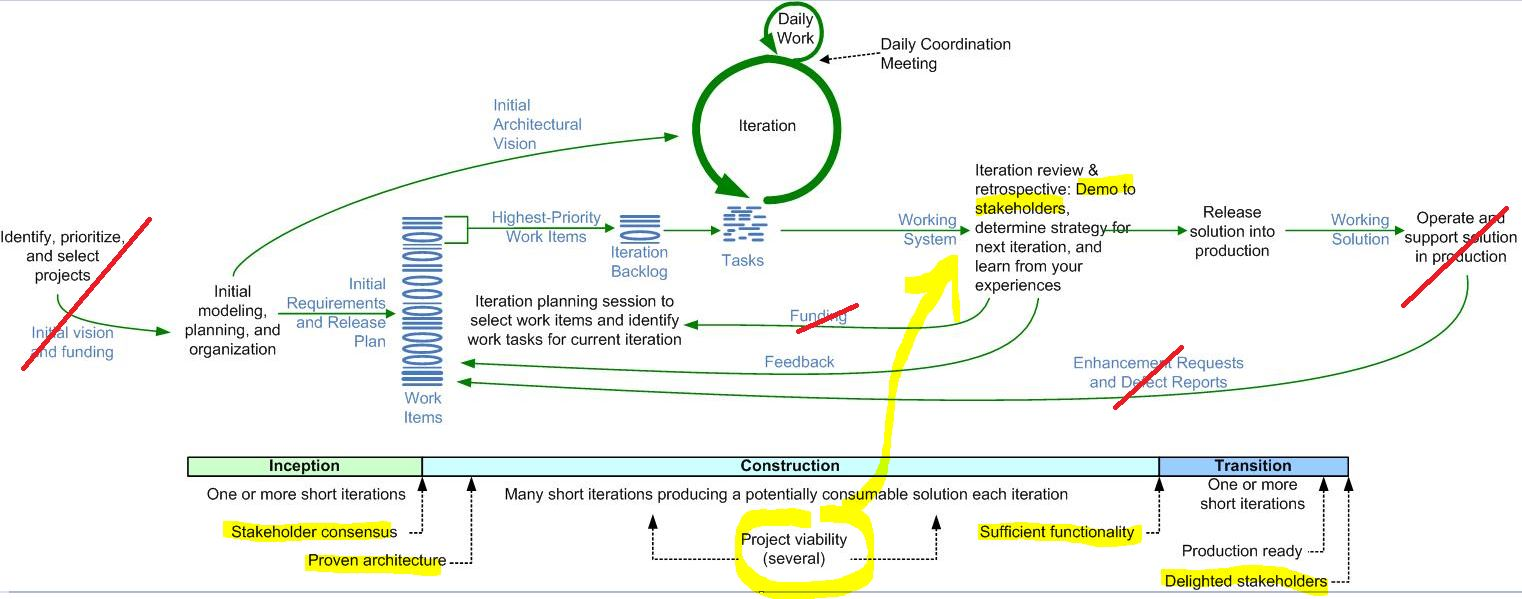
\includegraphics[width = .9\textwidth]{dadLifecycleUP2s}
\end{frame}
%%
%% This is part of quick-plan.tex
%%
\begin{frame}
    \section{Schedule}
\end{frame}


\end{document}
